\documentclass[14pt,a4paper]{book}
\usepackage[spanish,es-nodecimaldot]{babel}	% Utilizar español
\usepackage[utf8]{inputenc}					% Caracteres UTF-8
\usepackage{graphicx}						% Imagenes
\usepackage[hidelinks]{hyperref}			% Poner enlaces sin marcarlos en rojo
\usepackage{fancyhdr}						% Modificar encabezados y pies de pagina
\usepackage{float}							% Insertar figuras
\usepackage[textwidth=390pt]{geometry}		% Anchura de la pagina
\usepackage[nottoc]{tocbibind}				% Referencias (no incluir num pagina indice en Indice)
\usepackage{enumitem}						% Permitir enumerate con distintos simbolos
\usepackage[T1]{fontenc}					% Usar textsc en sections
\usepackage{amsmath}						% Símbolos matemáticos

\usepackage[table,xcdraw]{xcolor}
\setlength\headheight{26pt} 
\pagestyle{fancy}
\rhead{
\includegraphics[width=1cm]{./images/logo.png}}

% Comandos para poner el nombre de la asignatura
\newcommand{\asignatura}{Programación Lúdica}
\newcommand{\autor}{Carlos Nuñez Molina \\ Ignacio Vellido Expósito}
\newcommand{\titulo}{SynVic}
\newcommand{\subtitulo}{Game Description Document}

\begin{document}
    \pagenumbering{gobble}
    
% ==============================================================================
% Pagina de titulo
\begin{titlepage}
    \begin{minipage}{\textwidth}
        \centering

        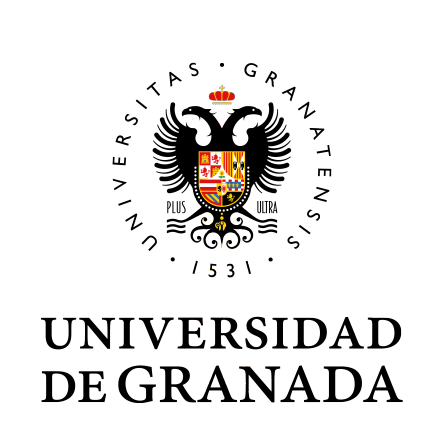
\includegraphics[scale=0.5]{images/ugr.png}\\

        \textsc{\Large \asignatura{}\\[0.2cm]}
        \textsc{GRADO EN INGENIERÍA INFORMÁTICA}\\[1cm]

        \noindent\rule[-1ex]{\textwidth}{1pt}\\[1.5ex]
        \textsc{{\Huge \titulo\\[0.5ex]}}
        \textsc{{\Large \subtitulo\\}}
        \noindent\rule[-1ex]{\textwidth}{2pt}\\[2.5ex]

        \end{minipage}

        \vspace{0.3cm}

        \begin{minipage}{\textwidth}

        \centering

        \textbf{Autores}\\ {\autor{}}\\[1.5ex]
        \vspace{0.2cm}

        
\includegraphics[scale=0.3]{images/etsiit.jpeg}

        \vspace{0.7cm}
        \textsc{Escuela Técnica Superior de Ingenierías Informática y de Telecomunicación}\\
        \vspace{1cm}
        \textsc{Curso 2019-2020}
    \end{minipage}
\end{titlepage}

% ==============================================================================
% ==============================================================================
    
    \pagenumbering{arabic}
    \tableofcontents
    \thispagestyle{empty}				% No usar estilo en la pagina de indice

    % ==============================================================================

    \chapter{Control de versiones}
\begin{table}[h]
	\centering
	\begin{tabular}{lllll}
		\cline{1-4}
		\multicolumn{1}{|l}{\cellcolor[HTML]{C0C0C0}\textbf{Versión}} & \cellcolor[HTML]{C0C0C0}\textbf{Fecha} & \cellcolor[HTML]{C0C0C0}\textbf{Autor} & \multicolumn{1}{l|}{\cellcolor[HTML]{C0C0C0}\textbf{Cambios}} &  \\ \cline{1-4}

		% -----------------
		\multicolumn{1}{|l}{1.0}	& 02/3/2020	& Ignacio & \multicolumn{1}{l|}{Primera versión}	&  \\ \cline{1-4}
		% -----------------
		\multicolumn{1}{|l}{1.1}	& 08/3/2020	& Carlos  & \multicolumn{1}{l|}{Añadida Ingeniera.}	&  \\ \cline{1-4}
		% -----------------
		\multicolumn{1}{|l}{1.2}	& 11/3/2020	& Ignacio & \multicolumn{1}{l|}{Añadido Bardo.}	    &  \\ \cline{1-4}
		% -----------------
		\multicolumn{1}{|l}{1.3}    & 24/3/2020 & Carlos  & \multicolumn{1}{l|}{Pulida la memoria antes de la entrega.}                   &  \\ \cline{1-4}
		% -----------------
		\multicolumn{1}{|l}{1.4}    & 09/4/2020 & Carlos  & \multicolumn{1}{l|}{Añadida descripción escenario DeathMatch.}                   &  \\ \cline{1-4}
		% -----------------
		\multicolumn{1}{|l}{1.5}    & 10/4/2020 & Carlos  & \multicolumn{1}{l|}{Añadida descripción control cámara.}                   &  \\ \cline{1-4}
		% -----------------
		\multicolumn{1}{|l}{1.6}    & 13/4/2020 & Carlos  & \multicolumn{1}{l|}{Añadida descripción escenario Captura.}                   &  \\ \cline{1-4}
		% -----------------
		\multicolumn{1}{|l}{1.7}    & 20/4/2020 & Carlos  & \multicolumn{1}{l|}{Añadido personaje Mago y eliminada mejora de habilidades.}                   &  \\ \cline{1-4}
		% -----------------
		\multicolumn{1}{|l}{1.8}    & 24/4/2020 & Carlos  & \multicolumn{1}{l|}{Corregida descripción Mago.} &  \\ \cline{1-4}
		% -----------------
		\multicolumn{1}{|l}{1.9}    & 10/5/2020 & Carlos  & \multicolumn{1}{l|}{Añadidos modelos 3D y actualizado el arte.} &  \\ \cline{1-4}		
		% -----------------
		\multicolumn{1}{|l}{1.10}    & 03/6/2020 & Carlos  & \multicolumn{1}{l|}{Actualizadas habilidades personajes.} &  \\ \cline{1-4}	
		% -----------------
		\multicolumn{1}{|l}{1.11}    & 04/6/2020 & Carlos  & \multicolumn{1}{l|}{Actualizado apartado de Gameplay y Mecánicas.} &  \\ \cline{1-4}	
		% -----------------
		\multicolumn{1}{|l}{1.12}    & 06/6/2020 & Carlos  & \multicolumn{1}{l|}{Actualizadas secciones 4, 5 y 6.} &  \\ \cline{1-4}	
		% -----------------
		\multicolumn{1}{|l}{1.13}    & 07/6/2020 & Carlos  & \multicolumn{1}{l|}{Actualizadas secciones 7, 8, 9 y 10.} &  \\ \cline{1-4}	
		% -----------------
		\multicolumn{1}{|l}{1.11}    & 08/6/2020 & Ignacio  & \multicolumn{1}{l|}{Retoques, formateo. Extendida explicación del networking.} &  \\ \cline{1-4}
		% -----------------
		% \multicolumn{1}{|l}{}       &           &         & \multicolumn{1}{l|}{}                   &  \\ \cline{1-4}
	\end{tabular}
	\caption{Control de versiones del documento}
	\label{table:cambios_doc}
\end{table}
	\chapter{Descripción del juego}

% ==============================================================================

\section{Características}
\subsection{General}
SynVic es un juego free-to-play de acción MOBA y perspectiva isométrica. En él los jugadores se enfrentan en partidas cortas mediante batallas 2vs2. Cada jugador elige el personaje con el que quiere jugar la siguiente partida y se le mete en un \emph{lobby} al azar con otros tres jugadores. De igual manera, se elige un mapa y objetivo al azar para esa partida, estando el objetivo asociado al mapa elegido. Una vez en el lobby, los jugadores toman parte en una votación para elegir a su compañero de equipo, teniendo en cuenta las habilidades de los distintos personajes y el objetivo de la partida.

\subsection{Multijugador}
El juego se centra en mapas 2vs2, con chat in-game y pre-game (en el lobby) para facilitar la cooperatividad. En el estado actual, no hemos implementado todavía el chat. En un futuro, se barajaría la adición de un sistema de chat de voz, si el chat de texto no fuera suficiente.

\vspace{\baselineskip}

También se incluye un sistema de clasificación de jugadores, separado en rangos, para facilitar un entorno competitivo para aquellos jugadores que lo deseen. De esta forma, serán emparejados con jugadores de su mismo nivel, haciendo que el \emph{match-making} sea justo. En la versión actual, no se ha implementado el sistema competitivo.

\subsection{Gameplay}
Queremos proporcionar una experiencia que sea a la vez dinámica, incluso caótica, y competitiva, centrada en la cooperación.

\vspace{\baselineskip}

La dinamicidad la proporcionamos mediante los elementos semi-aleatorios del juego, principalmente el \emph{match-making} aleatorio y la selección también aleatoria del mapa. Esto hará que cada partida sea diferente.

La cooperación la proporcionamos mediante las partidas 2v2. Los jugadores deben elegir bien a su compañero de equipo, estableciendo una estrategia para la victoria en función de la sinergias entre sus habilidades. Los diversos personajes del juego y sus habilidades estarán pensados para obligar a los jugadores a cooperar entre sí: un personaje tendrá un rol determinado y no será autosuficiente, de ahí la necesidad de cooperación.


% ==============================================================================

\section{Plataformas compatibles}
En principio nos centramos para las plataformas de PC Windows y Linux.

% ==============================================================================

\section{Público objetivo}
Nuestro público objetivo son jugadores jóvenes, de entre 12 y 35 años. Buscamos atraer, al mismo tiempo, jugadores acostumbrados a otros MOBA, que buscan una experiencia altamente competitiva, y a jugadores más \emph{casuals}, que buscan un juego con una curva de aprendizaje menos empinada que otros MOBA y donde poder disfrutar desde la primera partida.

% ==============================================================================

\section{Influencias}
Tomamos influencia de otros juegos del género MOBA (como \textit{Battlerite}, \textit{League of Legends} y \textit{DOTA2}) y derivados (como \textit{Overwatch}).

% ==============================================================================

\section{Cuestiones importantes}
% \subsection{¿De que va el juego?}
% \textit{En un párrafo, proporcionar una descripción general del juego.}

% \subsection{¿Cual es el objetivo principal del juego?}
% \textit{¿Que ha de conseguir el jugador dentro del juego para poder superarlo con éxito?.}

\subsection{¿Cuales son los aspectos diferenciadores del juego?}
% \textit{Con respecto a la competencia, ¿de que se diferencia nuestro juego?.}
En comparación con el resto de MOBAs, el juego se desmarca utilizando partidas cortas centradas en la cooperación. El hecho de que los jugadores seleccionen a su personaje sin conocer los personajes del resto de jugadores ni el objetivo de la partida hace que sea muy importante la capacidad de adaptación y cooperación con el compañero. Así, cada partida será diferente de la anterior y una nueva experiencia para el jugador.
	
% ==============================================================================

	\chapter{Gameplay y mecánicas del juego}

% ==============================================================================

\section{Gameplay}
\subsection{Núcleo}
% \textit{En pocos párrafos, detallar la esencia del juego. Estas palabras serán las semillas a partir de las cuales el diseño del juego irá creciendo, ayudando así a que el juego tenga bastante éxito en el mercado. El contenido de esta sección es similar a la del concepto del juego pero expresado de forma más esquemática, como un listado con viñetas.}

Para que este juego tenga éxito, debemos ser capaces de encontrar un equilibrio entre la parte dinámica/caótica y la parte competitiva.

\vspace{\baselineskip}

Por una parte, la parte dinámica/caótica viene dada por:
\begin{itemize}
  \item Partidas cortas.
  \item Elementos aleatorios: El jugador elige su personaje sin conocer el mapa/objetivo ni los personajes de los otros tres jugadores.
\end{itemize}

\vspace{\baselineskip}

Por otra parte, los siguientes elementos permiten a los jugadores habilidosos controlar y contrarrestar este ``caos'', proporcionando una experiencia competitiva: 
\begin{itemize}
  \item Los jugadores pueden votar para elegir a su compañero de equipo.
  \item Una vez elegidos los equipos, se pueden mejorar algunas habilidades para adaptar al personaje a la partida actual. En la versión actual, esta característica aún no está implementada.
  \item Los chats (lobby y in-game) permiten a los jugadores coordinarse con su compañero de equipo y establecer una estrategia, incluso antes de que empiece la partida.
\end{itemize}


\subsection{Desarrollo}

A continuación se detalla cómo se produce el desarrollo de una partida:
\begin{enumerate}
   \item El jugador elige el personaje con el que va a jugar la siguiente partida. No tiene control sobre cuál va a ser el mapa de la partida ni con qué otros jugadores será emparejado en el lobby, así que debe elegir el personaje simplemente en función de lo bueno que es con él o lo mucho que le apetece jugarlo.
   \item Pulsa en el botón \emph{Search Game} y empieza la búsqueda de partida. Una vez encontrados otros tres jugadores, se le mete en el lobby con los otros jugadores.
   \item Una vez en el lobby, forma parte de una votación para crear los equipos. Puede votar para que un jugador sea su compañero de equipo y votar a otro para que sea su oponente. Esta elección teóricamente debería hacerla en función de su personaje y el de los demás. Al jugador también se le da la posibilidad de no votar. Una vez que se ha acabado el tiempo o todos los jugadores han votado, se crean los equipos teniendo en cuenta las votaciones de los usuarios. Durante esta fase, en base al chat los distintos jugadores pueden discutir sobre los distintos equipos a formar.
   \item Una vez formados los equipos, los jugadores entran en un fase donde tienen que elegir hasta dos mejoras para sus habilidades, en función de los equipos formados. Durante esta fase, se sigue pudiendo usar el chat, pero ahora solo para hablar con el compañero de equipo. Esta fase no se ha implementado aún.
   \item Tras esta fase, empieza la partida propiamente dicha. Los jugadores compiten en equipos 2v2 (formados en el lobby) intentando alcanzar un objetivo que depende del mapa de la partida. El equipo que primero alcance el objetivo es el ganador y el otro es el perdedor.
   \item Cuando la partida termina, el jugador vuelve al menú principal. En función de si ha ganado o perdido, recibe puntos de experiencia para subir de nivel y monedas que puede usar para comprar nuevos personajes con los que jugar. Además, si la partida era competitiva, gana o pierde puntos de clasificación, según haya ganado o perdido, lo que influye en su puesto en la escalera clasificatoria.
\end{enumerate}

\subsection{Progresión}
% \textit{Trazar el flujo típico con una descripción detallada de lo que tiene que hacer el jugador para ir progresando en el juego e ir cumpliendo los objetivos. Si la sección anterior era la raíz de un árbol, esta sección constituye el tronco y las ramas.}
De cara a conseguir una mayor fidelización de los jugadores, se incluyen diversos sistemas de progresión. Por una parte, hay un sistema de progresión por niveles mediante los puntos de experiencia que se consiguen al jugar partidas. Este nivel refleja la experiencia que tiene un jugador dado, en función de la cantidad de partidas jugadas.

Por otra parte, los jugadores ganan monedas al jugar partidas, más en caso de victoria que de derrota. Estas monedas se usan para desbloquear personajes con los que jugar. De esta forma, el contenido del juego se va haciendo disponible poco a poco al jugador, en vez de todo de golpe, lo que podría abrumarlo y además no le daría ninguna sensación de progresión.

Por último, al jugar partidas clasificatorias, se ganan y pierden puntos según se ganen o pierdan partidas, respectivamente, y en función de estos se establece la posición del jugador en la escalera clasificatoria. Esto proporciona una experiencia competitiva y más "seria" para aquellos jugadores más "hardcore", que se tomen en serio el juego y que quieran mejorar.

\vspace{\baselineskip}

Estos sistemas de progresión no están implementados en la versión actual del juego.

% ==============================================================================

\section{Mecánicas}
\subsection{Movimiento}
Para moverse por el escenario del mapa, los jugadores harán uso de su ratón, como suele ser el caso en la mayoría de MOBA. Al hacer click con el botón derecho en un punto del suelo, el personaje caminará (con una velocidad que dependerá de cada personaje) hacia dicha posición a través del camino más corto.

\subsection{Acciones}
Aparte del movimiento, los jugadores tendrán a su disposición 5 habilidades adicionales, que dependerán del personaje escogido. 

Para realizar el ataque básico, se deberá posicionar el cursor sobre un enemigo y pulsar el botón derecho. Si el personaje se encuentra fuera del rango del ataque básico, se moverá hasta el límite de dicho rango y entonces atacará al enemigo. 

Para el resto de habilidades, habrá que pulsar la tecla del teclado correspondiente (Q, W, E o R) y, dependiendo de la habilidad en concreto, realizar alguna acción adicional, consistente en posicionar el cursor en algún punto del mapa y presionar de nuevo (una o varias veces) la misma tecla.

\subsection{Inteligencia Artificial}
En nuestro juego, hemos usado la inteligencia artificial para dos aspectos diferentes:

\vspace{\baselineskip}

Por una parte, cuando el jugador hace click en un punto del mapa, el jugador se mueve hacia dicho punto por el camino más corto. Para encontrar el camino más corto, hemos hecho uso de los nodos \emph{Navigation} y \emph{NavigationMeshInstance}, que proporciona Godot.

Por otra parte, en el mapa \emph{Captura}, hay un hada que se desplaza por el mapa. Este hada se va moviendo de forma semialeatoria de un punto a otro del mapa, siguiendo caminos ya preestablecidos, y priorizando unos lugares sobre otros. El funcionamiento concreto se explica en el apartado de Diseño de Niveles, en el subapartado del mapa \emph{Captura}.

%  ==============================================================================

\section{Configuración}
% \textit{Detallar si el juego ofrece la posibilidad al jugador de configurar ciertos aspectos del juego. Si esto es afirmativo, explicar qué es lo que se puede modificar y su accesibilidad (por ejemplo, si el juego admite configurar la resolución de pantalla, la calidad de los gráficos, etc.).}

Por ahora, hemos implementado el menú de configuración de sonido (ver figura \ref{fig:AudioMenu}). Este menú permite al usuario configurar de forma separada el volumen maestro (que afecta a todo el sonido del juego), el volumen de la música y el volumen de los efectos de sonido. Además, se puede directamente silenciar cada uno de estos volúmenes por separado.

\begin{figure}
	\centering
	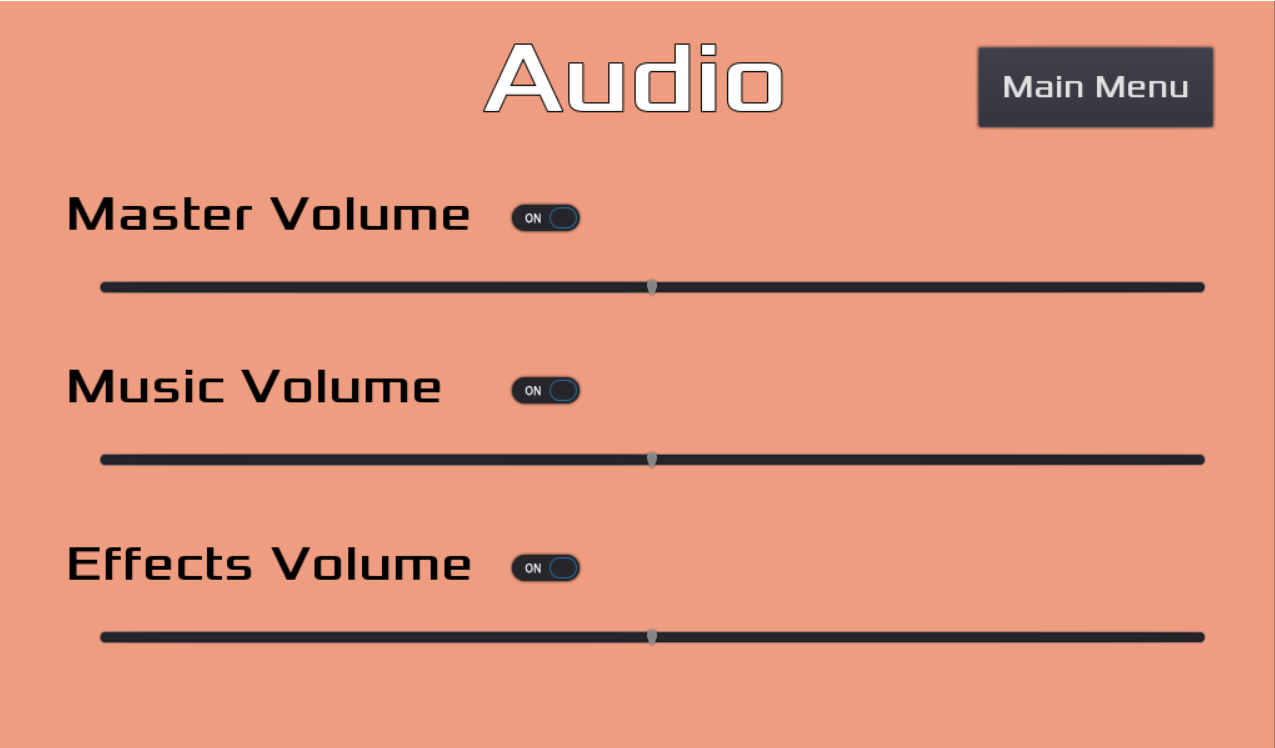
\includegraphics[width=0.8\linewidth]{figures/AudioMenu}
	\caption{Menú de configuración de sonido.}
	\label{fig:AudioMenu}
\end{figure}

\vspace{\baselineskip}

En el futuro, planeamos aumentar las opciones de configuración. Por un lado, habría que añadir una opción para configurar los controles y \emph{keybindings} (ej.: que se pueda lanzar una habilidad pulsando la tecla 1 en vez de Q). Por otro lado, habría que añadir un menú para configurar el apartado gráfico, para así permitir que aquellos jugadores con un PC de gama baja puedan jugar al juego con una buena tasa de FPS.

% ==============================================================================

\subsection{Modos de juego}
% \textit{Detallar los modos de juego que el usuario tendrá disponible. Para cada modo de juego, proporcionar una descripción detallada y si inicialmente es un modo que está bloqueado, incluir instrucciones para que el usuario sepa como tiene que desbloquearlo.}

Inicialmente se proponen los siguientes modos de juego, disponibles desde el primer momento (aunque el jugador no puede elegir cuál va a jugar en la próxima partida):
\begin{enumerate}
	\item \textbf{Deathmatch}: Modo 2vs2 en el que, para ganar, los jugadores de un equipo deberán matar 5 veces a los jugadores del otro equipo (puede ser 5 veces al mismo jugador o estar repartidas las muertes entre los dos jugadores enemigos). Cuando un jugador muere, \emph{respawnea}.
	
	\item \textbf{Captura}: Modo 2vs2 donde los jugadores deben defender una zona alrededor de un hada que se va moviendo por todo el mapa. Los equipos reciben puntos por cada jugador que esté dentro de la zona del hada en cada instante de tiempo. Una vez que han pasado 5 minutos, el equipo con más puntos gana. Cuando un jugador muere, \emph{respawnea}.
	
\end{enumerate}

\subsection{Arquitectura multijugador}
Para reducir al mínimo la latencia y simplificar el networking, se seguirá una esquema cliente-servidor, con servidor autoritario. Es importante evitar el envío de información redundante notificando únicamente de los cambios en el juego, es decir, el uso de actualizaciones en modo delta.

\vspace{\baselineskip}

La arquitectura se forma por un servidor autoritario, el cúal tienen su propia versión del juego, y se encarga de llevar la lógica. Cada jugador tiene la versión del cliente, la cuál durante la partida solo es responsable de actualizar la pantalla según los cambios indicados por el servidor y transmitir los comandos (ratón/teclado) introducidos por el usuario hacia este.
El servidor cuenta con una interfaz visual simple, permitiendo ver el estado de la partida con una representación gráfica simplificada.

El intercambio de mensajes se realizará usando la capa de networking que proporciona Godot, usando RTC con variantes TCP y UDP. El intercambio de mensajes continuos (donde se permite la pérdida de mensajes), como la posición de un personaje, se realizará mediante el protocolo UPD, y aquellos mensajes de gran importancia, como la notificación de crear un proyectil, harán uso de TCP.

Para no sobrecargar al servidor con entradas del usuario no válidas, el cliente también adicionalmente comprobará el estado de los cooldown antes de realizar las peticiones (pero manteniendo la responsabilidad de estos en el servidor para que no exista desfase entre ellos).

\vspace{\baselineskip}

Para un estado más avanzado del juego, sería recomendable fijar los envíos de mensajes en intervalos de tiempo concretos, reduciendo la latencia y estructurando el envío de mensajes. Esta técnica es usada en otros juegos del género asegurando la emisión de los paquetes a intervalos de frames regulares.
	\chapter{Interfaz de usuario}

% ==============================================================================

\section{Sistema visual}
\subsection{HUD}

El HUD se encuentra en pantalla durante todo el desarrollo de la partida. Se compone de 2 partes:

\subsubsection{Player HUD}
Incluye la vida del personaje y las habilidades, con su respectivo cooldown e información adicional, por ejemplo, si una habilidad se está \emph{casteando} (cargando para poder usarla) o si está \emph{activa} (tiene varios usos restantes antes de desactivarse y volver a ponerse en cooldown).

\begin{figure}[h]
	\centering
	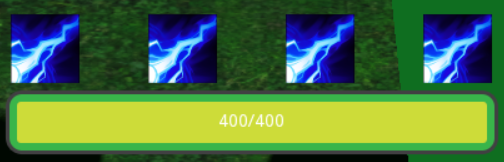
\includegraphics[width=0.8\linewidth]{figures/PlayerHUD}
	\caption{Habilidades del personaje y barra de vida.}
	\label{fig:PlayerHUD}
\end{figure}

\subsubsection{Match details}
En esta sección se muestra el estado actual de los objetivos de la partida. La información mostrada variará según el modo del juego, estos son:
\begin{itemize}
	\item \textbf{Deathmatch}: Se mostrará el número de vidas restantes de cada equipo.
	\item \textbf{Captura}: Se mostrará la puntuación de cada equipo así como el tiempo de partida restante (ver figura \ref{fig:MatchDetails}).
\end{itemize}

\begin{figure}[h]
	\centering
	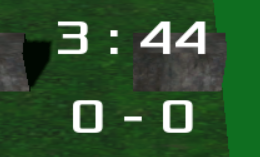
\includegraphics[width=0.8\linewidth]{figures/MatchDetails}
	\caption{Match Details del modo de juego \emph{Captura}.}
	\label{fig:MatchDetails}
\end{figure}

\subsection{Chat}
El juego tendrá dos chats: lobby y in-game. En la versión actual del juego, no hemos implementado todavía ninguno de ellos.

\vspace{\baselineskip}

El chat del lobby se podrá usar, antes de elegir equipo, para hablar con los otros tres jugadores (por ejemplo, para intentar "reclutar" a otro jugador con el que quieres jugar, antes de realizar la votación). Una vez que se ha votado y formado los dos equipos, se podrá usar el chat durante la fase de mejora de habilidades, pero solo para hablar con el compañero de equipo.

El chat in-game se podrá usar para hablar con el compañero de equipo durante toda la partida. Así, se proporciona al jugador una vía de comunicación para facilitar la cooperación.

\subsection{Menús}

\subsubsection{Menú principal}
El menú principal es lo primero que ve el jugador al entrar en el juego. Muestra la información del usuario (nombre, nivel y cantidad de monedas del juego de las que dispone (aunque todavía no hemos implementado nada de esto)) y diversos botones que permiten:

\begin{itemize}
	\item Ver el historial de partidas jugadas recientemente (no implementado). 
	\item Ver el puesto en la escalera clasificatoria (no implementado).
	\item Acceder a la configuración del juego (controles, audio y sonido). Por ahora, solo hemos implementado el menú de sonido (ver \emph{Menú de Sonido})
	\item Ver los amigos conectados (no implementado). El jugador puede agregar a otros jugadores dentro del juego para tenerlos en la lista de amigos y poder hablar con ellos. En el futuro, pensaremos en introducir algún modo de juego donde se pueda elegir jugar con/contra amigos.
	\item Acceder a la tienda del juego (no implementado). Aquí podrá comprar nuevos personajes, cosméticos, etc.
	\item Ver la información de los personajes (ver \emph{Menú de Personajes}).
	\item Buscar partida (al pulsar el botón \emph{Search Game}).
\end{itemize}

\begin{figure}[h]
	\centering
	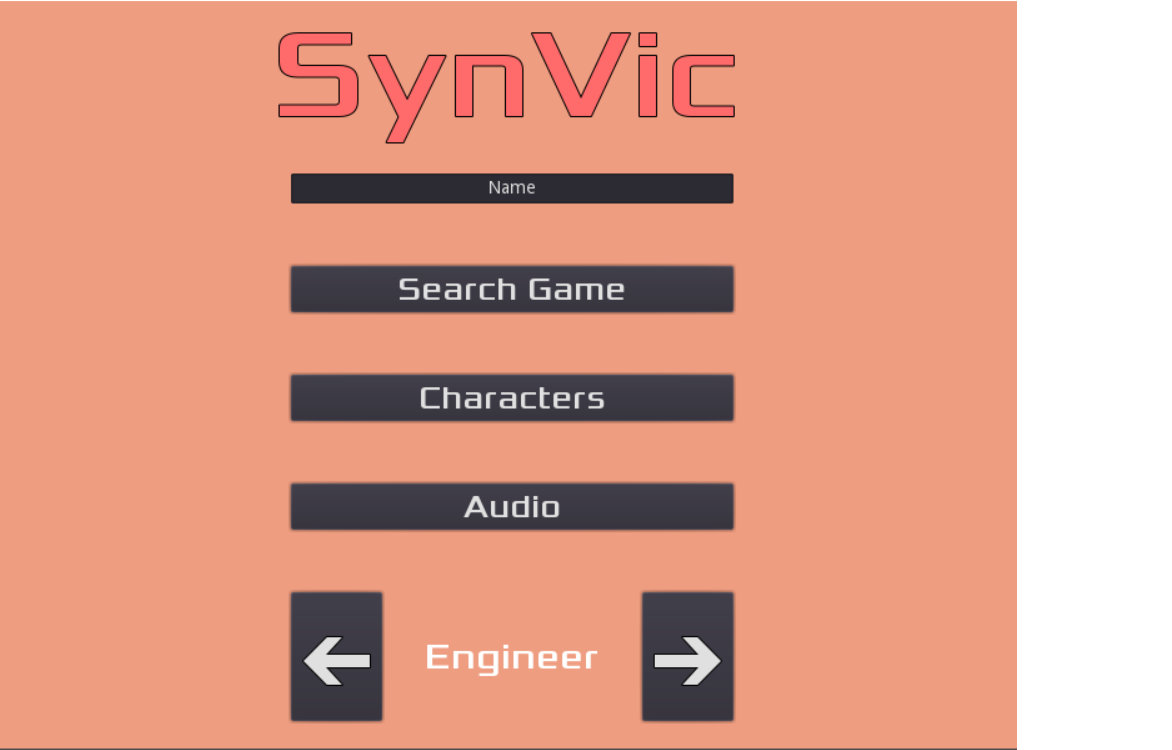
\includegraphics[width=0.7\linewidth]{figures/MainMenu}
	\caption{Menú principal del juego.}
	\label{fig:MainMenu}
\end{figure}

\subsubsection{Menú de Sonido}
Este menú permite al usuario configurar de forma separada el volumen maestro (que afecta a todo el sonido del juego), el volumen de la música y el volumen de los efectos de sonido. Además, se puede directamente silenciar cada uno de estos volúmenes por separado.

\begin{figure}[h!]
	\centering
	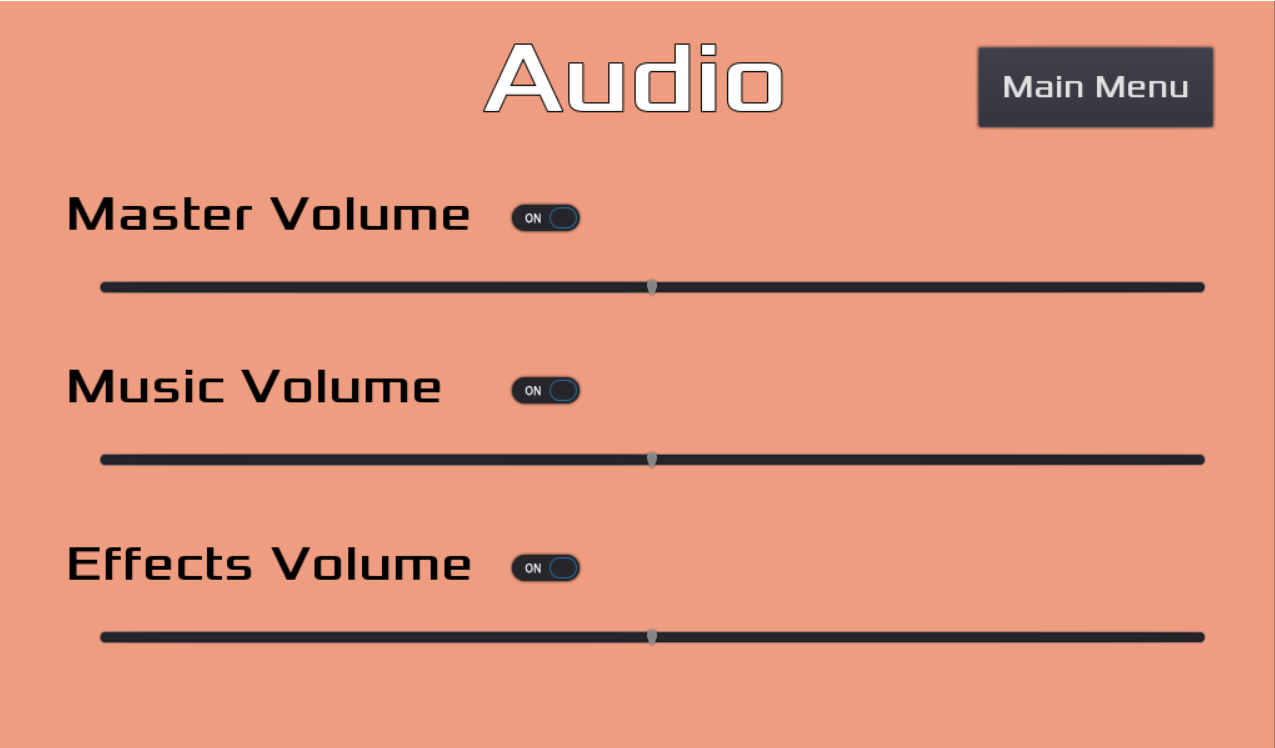
\includegraphics[width=0.7\linewidth]{figures/AudioMenu}
	\caption{Menú de configuración de sonido.}
	\label{fig:AudioMenu2}
\end{figure}

\subsubsection{Menú de Personajes}
En este menú, el jugador puede acceder a la información sobre cualquier personaje, incluyendo el funcionamiento de sus habilidades. De esta forma, el jugador puede informarse sobre lo que hace un personaje antes de jugar con él por primera vez.

\begin{figure}[h!]
	\centering
	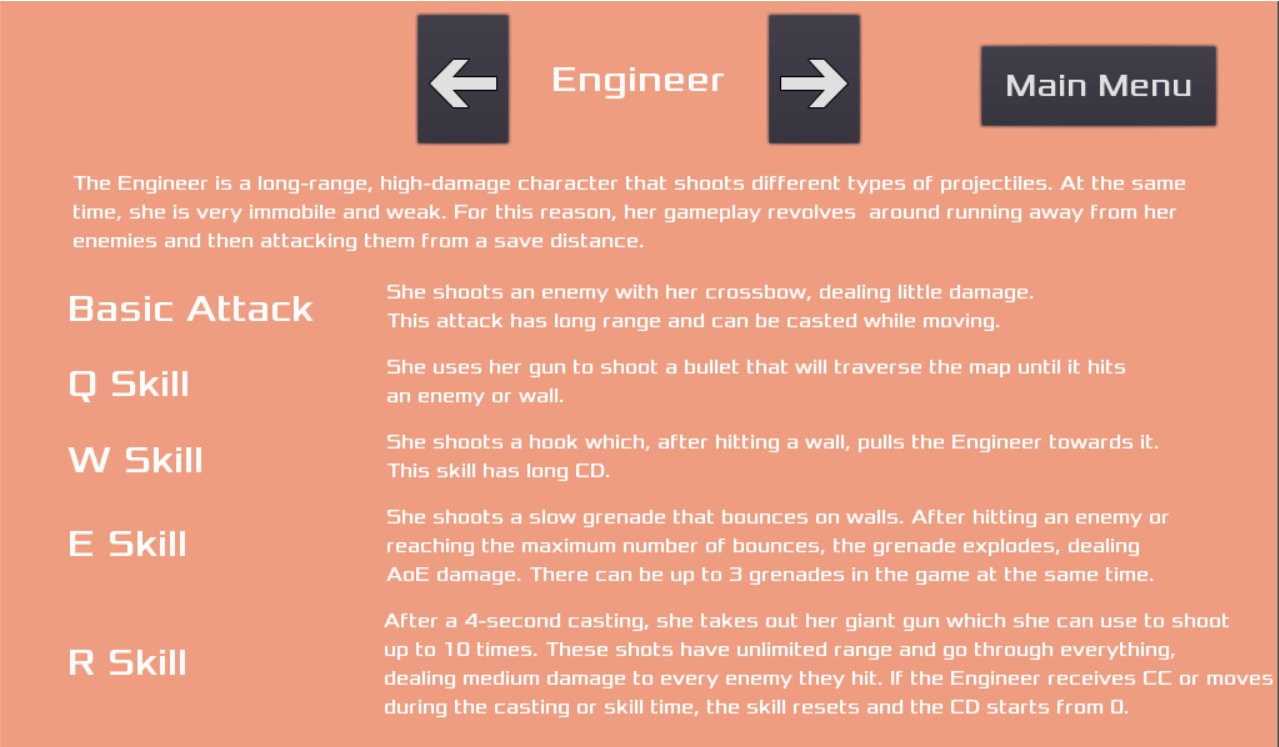
\includegraphics[width=0.7\linewidth]{figures/CharacterMenu}
	\caption{Menú de personajes.}
	\label{fig:CharacterMenu}
\end{figure}


\subsubsection{Lobby}
Tras encontrar una partida, el jugador accede al lobby junto a otros tres jugadores. Aquí, primero tendrá que votar para elegir a su compañero de equipo y, tras formar los equipos, elegir qué habilidades de su personaje mejorar (esto último todavía no está implementado).

\begin{figure}[h!]
	\centering
	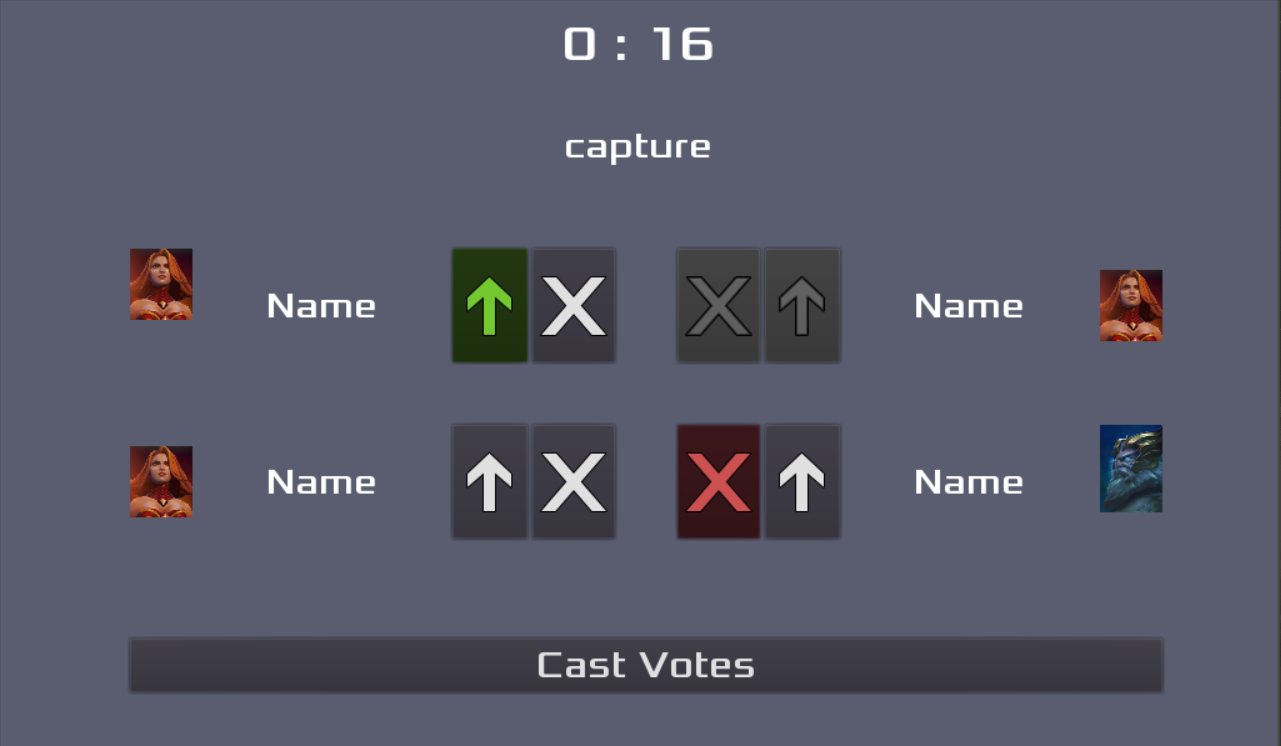
\includegraphics[width=0.7\linewidth]{figures/Lobby}
	\caption{Lobby.}
	\label{fig:Lobby}
\end{figure}

% ==============================================================================

\section{Sistema de control}
El juego usa un sistema de control por teclado y ratón. El usuario puede mover y rotar al personaje mediante clicks derechos del ratón. Si cliquea sobre un enemigo, el personaje aplicará un ataque básico sobre este.
Las teclas Q W E sirven para activar las tres habilidades básicas y la tecla R para la habilidad especial.

\vspace{\baselineskip}

La cámara del jugador tiene dos modos: \emph{auto} y \emph{manual}. En modo \emph{auto}, la cámara sigue el movimiento del jugador y siempre está centrada sobre este. En modo \emph{manual}, la cámara está fija y no sigue al jugador. En este modo, es el jugador el que debe mover la cámara arrastrando el ratón hacia los bordes de la pantalla. Al pulsar la tecla \emph{Space}, se cambia entre un modo y otro.
	\chapter{Arte y vídeo}

% ==============================================================================

\section{Objetivos}
% \textit{¿Qué se espera conseguir con el estilo del arte elegido? Por ejemplo, ¿se elige modelar en low poly para reducir presupuesto o meramente por cuestiones estéticas ya que esta muy relacionado con la temática del juego?}

El objetivo principal es utilizar un estilo artístico 3D parecido al de otros MOBA pero que sea lo más claro posible, de forma que no se distraiga al jugador con detalles.

También se pretende que el arte sea autodescriptivo, es decir, que a partir del modelo de un objeto este sea fácilmente reconocible y diferenciable del resto y que, incluso si un jugador nunca ha visto ese objeto antes, pueda hacerse una idea de lo que es a partir de su apariencia.

\vspace{\baselineskip}

Por la característica rápida del juego, se busca que haya contraste en los colores, de forma que se pueda diferenciar con claridad qué modelos hay en pantalla. Dotar a cada modelo de pocos colores (2 o 3 gamas) y remarcando los contornos debería ser una manera para conseguirlo fácilmente.

\vspace{\baselineskip}

Todo esto no solo se aplica a personajes y entornos, sino al diseño de los efectos y las interfaces que contenga el juego. Respecto al primero, será suficiente con mostrar que el efecto ha ocurrido, sin recurrir a ninguna manera vistosa de mostrarlo (por ejemplo, al impactar una habilidad o un golpe, el efecto debería ser lo menos disruptivo visualmente posible). En la medida de lo posible, evitar de la dependencia de los efectos de sonido, se pretende que el juego sea autodescriptivo sin necesidad de usar audio.

\section{GUI}
% \textit{Ventanas, punteros, marcadores, íconos, botones, menús, etc. Todos estos elementos deben recogerse en esta sección, con una descripción de para que se utilizan y una representación gráfica de ellas. }
El diseño de la GUI cumplirá lo mencionado anteriormente. Será simple (incluso minimalista) y muy descriptiva, mostrando al jugador de manera rápida y sencilla la información que necesite, sin distraerlo con detalles innecesarios.
	
\section{Decorados}
% \textit{Decorados de terreno, texturas, skyboxes, fondos, tiles... Todos estos elementos deben recogerse en esta sección, con una descripción de para que se utilizan y una representación gráfica de ellas. }
    
Se utilizará una cámara isométrica que no se puede rotar, por lo que no se verán las caras "traseras" de los decorados. A pesar de esto, los obstáculos y decorados, al igual que los personajes, serán 3D.

Respecto a los fondos, se usarán skyboxes de la temática del escenario. Por ejemplo, para el escenario del modo Capture que está ambientado en un bosque, el skybox representará un bosque. Por ahora, como placeholders, los fondos son simplemente de un color plano, de acuerdo a la temática del escenario.

\section{Personajes y Habilidades}
% \textit{Animaciones de enemigos y jugadores (sprites o modelos), objetos, armas, power-ups, etc. Todos estos elementos deben recogerse en esta sección, con una descripción de para que se utilizan y una representación gráfica de ellas. }
Los modelos de los personajes serán 3D, como el resto de modelos. Tal y como hemos mencionado, estos modelos serán simples, usando pocos colores y sin tener demasiados detalles, para no distraer a los jugadores del gameplay. A pesar de su simpleza, debe ser fácil diferenciar un personaje de otro. Para ello, los modelos deben ser "eficaces", es decir, ser capaces de transmitir la "esencia" del personaje de forma directa y sencilla, sin tener que usar detalles. Como cada personaje se basa en una idea sencilla (por ejemplo, la ingeniera es una mujer, pequeña, que usa diversas armas y pistolas mucho más grandes que ella), el modelo debe centrarse en estos aspectos, transmitiendo al jugador la idea en la que se basa el personaje. De esta forma, conseguiremos que los modelos sean a la vez sencillos y autodescriptivos.

\vspace{\baselineskip}

Los efectos de las habilidades también seguirán esta filosofía del minimalismo, aún más si cabe. Intentaremos no abusar de los efectos y solo usarlos cuando sean necesarios para mostrar algún tipo de información al usuario. Por ejemplo, los usamos en la ulti del mago (aunque, en este momento del desarrollo, usamos un círculo en vez de un sistema de partículas) para mostrar el rango de acción de su habilidad y permitir a los jugadores enemigos que escapen de dicha área. Cuando usemos efectos, intentaremos que sean simples para que no abrumen al jugador ni lo distraigan de la acción.
	\chapter{Sonido y música}

% ==============================================================================

\section{Objetivos}
% \textit{Objetivos técnicos y estéticos para la parte sonora del juego. Describir las emociones que se pretenden inducir al jugador. Nombrar juegos existentes o películas como ejemplos para detallar mejor esta sección.}	

El sonido y la música del juego, de la misma forma que el arte, va a ser minimalista y sencillo, para no distraer al jugador, centrándose en cumplir un objetivo concreto. 

El objetivo de la música es el de la ambientación e inmersión, en función de cada mapa concreto. El objetivo de los efectos de sonido es aportar cierta información adicional al usuario, complementando la información visual que recibe el jugador. Aun así, hemos diseñado el juego para que sea factible jugarlo sin sonido (aunque no sea aconsejable).


% ==============================================================================

\section{Efectos de sonido}
\subsection{GUI}
Al pulsar un botón, se reproducirá un sonido que funcionará como feedback para el jugador. De la misma forma, se reproducirá un sonido que avisará al jugador cuando se haya encontrado partida. En el futuro, quizás añadamos más sonidos.

Por ahora, no hemos añadido todavía ningún sonido de la GUI.
	
\subsection{Efectos especiales}
Las habilidades tienen un efecto especial de sonido que se reproduce cuando se usan. Este sonido es diferente para cada habilidad del juego de forma que, a partir solo del sonido, un jugador avanzado podrá saber qué habilidad se ha usado. De la misma forma, el sonido es 3D, con lo que se podrá averiguar desde dónde se ha lanzado la habilidad, incluso si el jugador que la ha usado se encuentra fuera del campo de visión del jugador. Algunas habilidades tienen efectos de sonido adicionales. Por ejemplo, la habilidad \emph{E} de la ingeniera lanza una granada que, cuando explota, emite también un sonido.

% ==============================================================================

\section{Música}
El objetivo de la música, a diferencia de los efectos de sonido, no tiene nada que ver con el gameplay, al menos directamente. La música sirve de ambientación, ayudando a la inmersión del jugador en el juego. Cada mapa (y su modo de juego asociado) tiene un tema diferente, que se reproduce en bucle durante toda la partida al menos que el jugador haya desactivado la música. Este tema será simple (para no distraer al jugador) y estará asociada a la estética del mapa, reforzando la temática de este. Por ejemplo, como el mapa del modo de juego \emph{Captura} es un bosque, el tema de dicho mapa tendrá como temática la naturaleza.

	\chapter{Diseño de niveles}

% ==============================================================================

\section{DeathMatch}
El escenario para el modo de juego \emph{DeathMatch} se caracteriza por motivar el enfrentamiento entre los dos equipos. Tiene unos pocos obstáculos que proporcionan cobertura a los jugadores pero, al ser pequeño, evita que los jugadores huyan indefinidamente. Además, tiene forma octogonal y es simétrico, tanto horizontal como verticalmente. En los límites del escenario hay paredes invisibles que funcionan como cualquier otro obstáculo. En la figura \ref{fig:DeathMatchStage} se muestra una captura del escenario:

\begin{figure}[h]
	\centering
	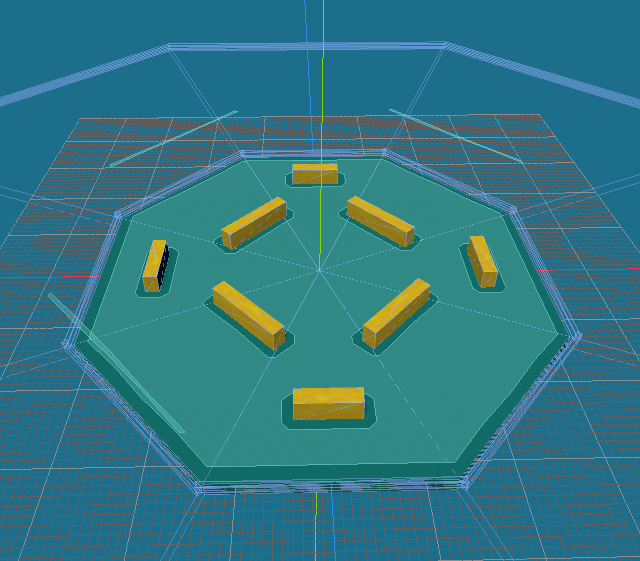
\includegraphics[width=0.8\linewidth]{figures/DeathMatchStage.png}
	\caption{El escenario para el modo de juego DeathMatch.}
	\label{fig:DeathMatchStage}
\end{figure}

\section{Captura}
Este mapa es más grande que el del modo \emph{DeathMatch}. Hay cinco puntos de interés, llamados \emph{fortalezas}: la del centro y una para cada esquina. En este modo de juego, el hada (que empieza en el punto central) va moviéndose de una fortaleza a otra de la forma siguiente: cuando acaba de llegar a una fortaleza, permanece inmóvil durante un periodo de tiempo muestreado a partir de una distribución uniforme en $[15, 25]$ segundos; una vez se termina este tiempo, elige una fortaleza nueva (que no puede ser ni la misma ni, en el caso de estar en una esquina, la esquina opuesta); en el caso de las esquinas, la fortaleza del centro es el doble de probable; tras elegir la fortaleza, empieza a dirigirse hacia ella por un camino predefinido y se repite este proceso indefinidamente. 

\vspace{\baselineskip}

El mapa tiene tres tipos de zonas: la fortaleza central, las fortalezas de las esquinas y las zonas \emph{de paso}. Las fortalezas de las esquinas son fáciles de defender, al tener solo dos aperturas. La fortaleza central es más difícil de defender, al tener cuatro aperturas. Las zonas \emph{de paso}, por las que se mueve el hada de una fortaleza a otra, son zonas abiertas por lo que, sumado al hecho de que el hada se va moviendo, son muy difíciles de defender. De esta forma, al haber tres tipos de zona y cada una con una dificultad diferente de cara a ser defendida, esperamos dar dinamicidad a la partida y evitar que ciertos tipos de personajes (principalmente aquellos que pueden poner muros o tienen ataques de largo alcance pero poca movilidad) tengan una ventaja injusta sobre el resto de personajes.

\begin{figure}[h]
	\centering
	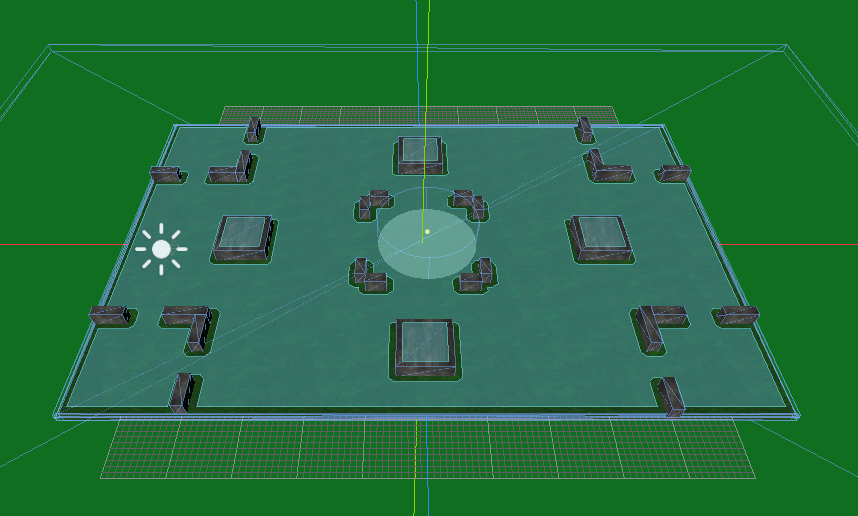
\includegraphics[width=0.8\linewidth]{figures/CaptureStage.png}
	\caption{El escenario para el modo de juego Captura.}
	\label{fig:CaptureStage}
\end{figure}
	\chapter{Diseño de personajes}

% ==============================================================================

\section{Ingeniera \emph{(Nombre Provisional)}}

\subsection{Gameplay}
La ingeniera es un personaje que se especializa en el ataque a larga distancia mediante diversos tipos de proyectiles. Es un personaje que aporta una gran cantidad de daño y desde una distancia de seguridad a costa de tener poca vida y movilidad.

Para ser efectivo con ella, el jugador debe hacer todo lo posible por
alejarse cuanto más pueda de los enemigos y, entonces, atacarlos aprovechándose de su gran rango. Como la ingeniera solo tiene una habilidad para escapar del peligro, su $W$, sus habilidades requieren que se quede inmóvil para usarlas y tiene poca vida, esto hace que sus opciones de supervivencia sean muy limitadas si los enemigos consiguen cubrir la distancia que los separa. De esta forma, el gameplay de la ingeniera consiste en alejarse de los enemigos, atacarlos desde un lugar seguro y repetir este proceso cada vez que los enemigos consiguen acercarse.

\subsection{Habilidades}
\subsubsection{Habilidades básicas}
\begin{itemize}
\item \textbf{Ataque Básico.} Al hacer click en un enemigo le dispara con una ballesta. El disparo hace poco daño pero tiene bastante rango. Es la única habilidad que no necesita que se quede quieta para usarse.
\item \textbf{Q.} Saca una pistola y dispara un proyectil de alcance infinito pero que no atraviesa obstáculos.
\item \textbf{W.} Dispara un gancho de alcance medio que, al impactar con un obstáculo, lleva a la ingeniera hasta este. Para limitar sus opciones de movilidad, el CD de esta habilidad es elevado.
\item \textbf{E.} Dispara una granada. Esta granada es un proyectil lento que rebota con los obstáculos un número limitado de veces. Tras chocar con un enemigo o alcanzarse el número máximo de rebotes, la granada explota, infringiendo daño en un área pequeña. El número máximo de granadas que puede haber en un momento dado en el mapa es de 3.
\item \textbf{Ultimate (R).} Saca una pistola gigante que tiene un tiempo de carga de 4 segundos antes de poderse usar. Una vez que ha terminado el tiempo de carga, puede realizar 10 disparos en rápida sucesión que tienen alcance ilimitado y atraviesan todos los obstáculos y enemigos, causando daño moderado a los enemigos contra los que impactan. Durante todo el proceso que dure la habilidad, la ingeniera no puede moverse del sitio. Si recibe crowd control (CC) durante el tiempo de carga o de uso de la habilidad, la habilidad se cancela, con lo que puede volver a moverse. También puede elegir cancelar la habilidad en cualquier momento de carga o uso. Al cancelarse, la carga de la ulti vuelve a 0. Esta habilidad tiene un CD largo.
\end{itemize}

\subsection{Diseño}

\begin{figure}[h]
	\centering
	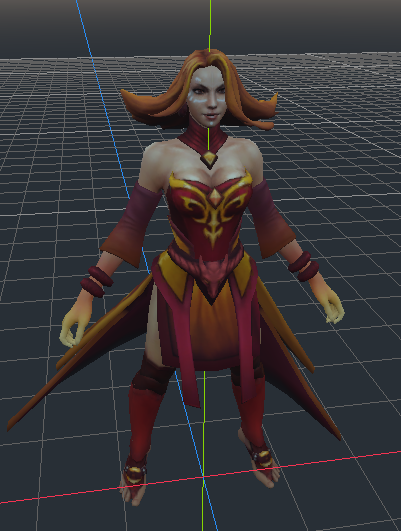
\includegraphics[width=0.6\linewidth]{figures/EngineerModel.png}
	\caption{Modelo Provisional de la Ingeniera.}
	\label{fig:EngineerModel}
\end{figure}

La ingeniera es una chica de complexión pequeña que lleva a la espalda una mochila, demasiado grande para ella, con todos los artilugios que usa para la batalla. El diseño del personaje está construido alrededor de este contraste, personaje pequeño con herramientas demasiado grandes para ella. Además, debido al gran peso de su mochila, se justifica que la ingeniera sea lenta y deba pararse siempre que usa una habilidad, debido al gran peso de las armas y a su difícil manejo. La ingeniera tiene también el pelo largo para enfatizar todavía más este contraste.

Este personaje estaría inspirado en el arquetipo ingeniero/artificiero de otros juegos. Como traje, llevaría un mono simple de trabajo y, aparte, unas gafas sobre la cabeza de estilo SteamPunk. El diseño de personaje debe transmitir que la ingeniera es un personaje muy inteligente que se ha valido de su gran inteligencia y habilidad para crear un gran conjunto de armas pero que, debido a su poca fuerza física y su torpeza, le cuesta usar sus propias creaciones.

En la figura \ref{fig:EngineerModel} se puede ver el modelo de la ingeniera que hemos usado como \emph{placeholder} (modelo provisional) para este proyecto. Este modelo es el del personaje \emph{Lina} del videojuego Dota 2, que se ha descargado de la siguiente página: \emph{http://www.dota2.com/workshop/requirements}.

\subsection{Sonido}
Los efectos de sonido de las habilidades de la Ingeniera están asociados a disparos, tanto de pistolas como de arcos y otras armas. Aparte, su ultimate tiene un sonido de carga, que se reproduce durante los 4 segundos que dura el casteo.

% --------------------------------------------------------------

\section{Bardo \emph{(Nombre Provisional)}}

\subsection{Gameplay}
El bardo es un flautista support caracterizado por aplicar buffos en areas de efecto alrededor suya. Apenas aporta daño al equipo pero aumenta las capacidades de supervivencia de este.

El bardo cuenta con un sistema de recursos: Melodías. Cada habilidad básica genera una melodía que se va almacenando hasta un máximo de 3. Estas melodías se pierden cuando el bardo sufre una cierta cantidad de daño o CC. Una vez se alcanza el máximo de melodías, la producción de otra elimina la primera de ellas.
Las melodías mejoran los stats de la habilidad que la producen y aplica un efecto temporal en el ataque básico (esto último es importante porque sino un healer y un tanque no tienen mucha viabilidad y están condenados desde el primer momento), y pueden ser descargados en la R para generar un gran área de efecto con efectos especiales. Los stats también se acumulan según el número de melodías.

La forma de jugar del bardo es cerca de su aliado, protegiendo y eligiendo cuidadosamente la melodías que desea mantener. Puesto que los efecctos de la R dependen de las últimas 3 melodías, y que el casting de estas lleva su tiempo, debe tener buena visión de futuro sobre la situación del juego a la que se va a enfrentar.

\subsection{Habilidades}
\subsubsection{Habilidades básicas}
Q-W-E tienen un cooldown medio (ej: 5s) y mientras se utilizan el bardo no puede atacar (pero sí moverse). Durante la duración de la habilidad se aplica el efecto, una vez acaba desaparece (excepto los stats de las melodías). La R tiene un cooldown bajo para una habilidad final (ej: 20 s), y se aplica inmediatamente tras un pequeño casting.

\begin{itemize}
    \item \textbf{Ataque Básico.} Dispara un dardo con la flauta. Mantiene un rango relativamente alto pero con muy poco daño. Poca velocidad de disparo.
    \item \textbf{Q.} Cura durante unos segundos alrededor suya. Sus básicos adquieren robo de vida.
    \item \textbf{W.} Aumenta la velocidad de ataque y de movimiento de los aliados en el área.
    \item \textbf{E.} Aumenta el daño básico de los aliados en el área.
    \item \textbf{Ultimate (R).} Descarga las melodías almacenadas en un gran área de efecto alrededor suya. Si el bardo no tiene 3 melodías en ese momento únicamente se juntan los efectos de las que haya, en caso de que haya 3:
    \begin{itemize}
        \item Q-Q-Q: Cura al máximo y revive a los aliados en el área. (El revivir puede estar demasiado roto, quizás transformarlo por: aumentar la vida máxima de los personajes temporalmente)
        \item W-W-W: Aumenta en gran medida la velocidad de ataque y de movimiento y de aliados. Durante ese tiempo pueden atravesar unidades (quizás no es muy fuerte)
        \item E-E-E: Los enemigos reciben más daño durante los siguientes segundos.
        \item Q-W-E: Stunea a todos los enemigos de la zona durante unos segundos.
        \item Q-Q-W: Por decidir.
        \item Q-Q-E: Por decidir.
        \item W-W-Q: Por decidir.
        \item W-W-E: Por decidir.
        \item E-E-Q: Por decidir.
        \item E-E-W: Por decidir.
    \end{itemize}
\end{itemize}

\subsection{Diseño}
Podría orientarse como un flautista de Hamelín con un toque más misterioso. Podría llevar capa y una bolsa de la que sobresalen partituras. Puesto que dispara dardos, podrían salirle de un compartimento que tenga en el brazo.

Las áreas de efecto de las habilidades deberían diferenciarse con claridad (podrían estar acompañadas con dibujos de notas musicales, aunque quizás sobrecargue demasiado). Sería recomendable que cada una se asociase con un color primario diferente (pero con cuidado con no saturarse con el terreno). Las ultis podrían separar el área en diferentes colores según las habilidades o podrían consistir de la combinación de sus colores.

\subsection{Sonido}
Cada habilidad debería producir una melodía diferente (preferiblemente de flauta). De la misma manera cada versión de la R vendría acompañada de un sonido diferente (preferiblemente con orquestación)

% --------------------------------------------------------------

\section{Mago \emph{(Nombre Provisional)}}

\subsection{Gameplay}
El mago es un personaje de apoyo que se especializa en el control del mapa, proporcionando protección a su aliado y evitando que los enemigos puedan llegar hasta él. Al contrario que en otros juegos, es bastante \emph{tanque}, lo que le permite preocuparse menos por su seguridad centrándose casi por completo en mantener a su aliado vivo y en darle apoyo.

Sus habilidades giran entorno al control del mapa y al posicionamiento de los distintos jugadores: él, su aliado y el equipo enemigo. Debe mantener alejado a su aliado del equipo enemigo, de ahí que tenga especial sinergia con campeones frágiles y/o con poca movilidad que tienen ataques a larga distancia. Su posicionamiento, en cambio, debe ser totalmente opuesto. Debido a sus habilidades y a su gran aguante, debe intentar siempre ``estar en medio'' del equipo enemigo, molestándolos e impidiéndoles llegar hasta su aliado.

\subsection{Habilidades}
\subsubsection{Habilidades básicas}
\begin{itemize}
\item \textbf{Ataque Básico.} Al hacer click en un enemigo le da un golpe con su bastón. Este ataque, de corto alcance, hace muy poco daño pero invoca al hielo para aplicar una ralentización pequeña durante un periodo de tiempo medio.
\item \textbf{Q.} Invoca un elemento al azar sobre una zona. Los enemigos que pasen sobre esa zona recibirán un debuff que dependerá del tipo de elemento. De la misma forma, los proyectiles aliados que pasen sobre esa zona aplicarán el mismo debuff al impactar. Los elementos y sus debuffs asociados son: hielo - ralentización, fuego - daño por segundo, veneno - vulnerabilidad (aumenta el daño recibido por los siguientes ataques). Para usar esta habilidad, el jugador debe poner el ratón en la zona donde quiere castearla y pulsar la tecla \emph{Q}.
\item \textbf{W.} Intercambia su posición por la de su aliado.
\item \textbf{E.} Levanta un muro de piedra en la posición deseada. El funcionamiento es el siguiente: el jugador debe pulsar la tecla \emph{E} en un punto y después volver a pulsarla con el ratón en otro punto, para crear un muro que vaya de un punto al otro. Si ambos puntos están demasiado lejos entre sí, el muro será desde el primer punto hacia el segundo punto pero se \emph{cortará} antes de llegar a este último. De la misma forma, si ambos puntos están demasiado cerca, no se construirá el muro porque sería demasido pequeño. El muro permanece en el mapa hasta que el jugador construye otro.
\item \textbf{Ultimate (R).} Tras un largo tiempo de casteo (que no puede cancelar y durante el cual no puede ejecutar ninguna acción ni moverse) invoca a una tormenta que \emph{stunea} a los enemigos en una zona alrededor suya. Estos enemigos no podrán moverse ni realizar ninguna otra acción durante 5 segundos (tiempo de duración del \emph{stun}).
\end{itemize}

\subsection{Diseño}

\begin{figure}[h]
	\centering
	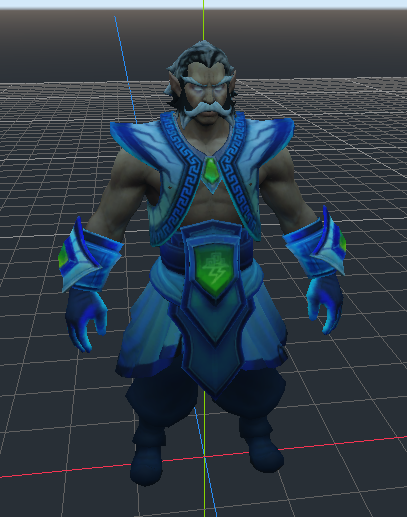
\includegraphics[width=0.6\linewidth]{figures/MageModel.png}
	\caption{Modelo Provisional del Mago.}
	\label{fig:MageModel}
\end{figure}

El mago es un hombre de complexión fuerte que está ataviado con una túnica y un gran bastón mágico, que usa para todos sus ataques. Al igual que la ingeniera, este personaje también se basa en un contraste: fuerza vs inteligencia, físico vs mental. Por una parte, este personaje es fuerte. Su misión es \emph{tanquear} al equipo enemigo mientras protege a su aliado. Por otra parte, al ser un mago, todas sus habilidades (menos su ataque básico) giran alrededor de su magia. Su diseño debe reflejar este contraste, manteniendo a la vez un equilibrio entre ambas facetas.

Todas sus habilidades usan/invocan algún elemento. Su ataque básico usa hielo. Su \emph{Q} usa hielo, fuego o veneno, según el efecto escogido al azar. Su \emph{W} usa aire (teletransportación). Su \emph{E} usa tierra (invoca un muro de roca). Su \emph{R} usa rayo (invoca una tormenta).

En la figura \ref{fig:MageModel} se puede ver el modelo del mago que hemos usado como \emph{placeholder} para este proyecto. Este modelo es el del personaje \emph{Zeus} del videojuego Dota 2, que se ha descargado de la siguiente página: \emph{http://www.dota2.com/workshop/requirements}.

\subsection{Sonido}
Los efectos de sonido de las habilidades del Mago están asociados a magia y elementos (como el sonido de tormenta que se reproduce cuando activa su ultimate). Además, mientras castea su ultimate, se reproduce un efecto de sonido que avisa a los enemigos de que se tienen que alejar del Mago para no ser stuneados.
	\chapter{Implementación}
\section{Metodología de desarrollo}
Empezamos siguiendo una metodología parecida a Scrum: establecimos una serie de objetivos globales e íbamos estableciendo objetivos semanales, que a su vez influían en los globales. Sin embargo, nos dimos cuenta de que, al ser solo dos personas en el equipo y hablar casi todos los días por Telegram, no era necesario seguir una metodología Ágil en concreto. Simplemente, nos dividimos las tareas que teníamos que hacer desde ese momento hasta la entrega del proyecto y fuimos trabajando en ellas a nuestro ritmo. Cuando terminábamos una tarea, se lo decíamos a nuestro compañero y valorábamos el resultado entre los dos. En el caso de que se nos ocurrieran nuevas tareas que hacer (como solucionar un nuevo bug), lo hablábamos con el otro y lo añadíamos como nueva tarea a realizar.

\section{Engine}
% \textit{Una descripción detallada del engine que se está usando para desarrollar el juego. En todo caso, detallar la versión utilizada, su página web, si es un engine propio o de terceros, etc.}

Se está utilizando el motor Godot en su versión 3.2, ya que es un motor de juegos sencillo de usar a la vez que completo. El lenguaje de programación usado es el lenguaje de scripting propio de Godot, GDScript. Hemos usado este lenguaje de programación porque es rápido de programar (se parece a Python, con el cuál ambos tenemos experiencia) y fácil de integrar con Godot.
	
\section{Tecnologías empleadas}
Como repositorio para los archivos del juego, hemos usado Git y GitHub. Hemos decidido usar esta tecnología principalmente por dos razones:

\begin{itemize}
	\item \textbf{Seguridad}. Al tener un repositorio en GitHub, tenemos la certeza de que, en caso de que los repositorios locales en nuestros ordenadores se perdieran, siempre podremos recuperar los archivos del juego desde GitHub.
	\item \textbf{Facilidad de desarrollo}. Gracias a esta tecnología, nos ha resultado sencillo trabajar los dos en el mismo proyecto. Simplemente, cada vez que uno realizaba un cambio, hacía \emph{push} a GitHub y el otro hacía \emph{pull} desde GitHub, para seguir trabajando en el proyecto.
\end{itemize}

Aparte, también hemos utilizado la opción que da GitHub (en la pestaña \emph{Projects}) para crear un tablero Kanban, donde se pueden añadir tarjetas en columnas indicando las tareas por hacer, en progreso y terminadas.
	\chapter{Monetización}
\section{Modelo de monetización}
SynVic es un juego free-to-play, sin ningún carácter pay-to-win. Esto significa que ningún elemento que los jugadores puedan comprar con dinero real dará ninguna ventaja sobre el resto de jugadores. Por tanto, los jugadores podrán comprar:

\begin{itemize}
	\item Aspectos para los personajes (\emph{skins}). Estos aspectos harán que los personajes se vean de manera diferente, sin impactar de ninguna forma en el gameplay.
	\item Personajes adicionales. Estos personajes se podrán desbloquear con el dinero del juego obtenido al jugar partidas. No obstante, los jugadores más impacientes también podrán decidir comprar estos personajes con dinero real.
\end{itemize}

Posteriormente, barajaremos la posibilidad de añadir más elementos de compra, como \emph{lootboxes} o imágenes y fondos de perfil.

    \setlength{\parskip}{1em}
    
    % ==============================================================================
    
    % \newpage
    % \bibliography{bibliografia}
	% \bibliographystyle{plain}
\end{document}


\end{document}